\section{Реализация алгоритма}
\label{}

Требования, предъявленные к разрабатываемому исполняемому файлу:
\begin{enumerate}
\item Время исполнения для предоставленных файлов-примеров имеет порядок секунд или минут. Возможность работы в реальном времени не требуется.
\item Целевая платформа --- Microsoft Windows. Доступны инструменты .NET Framework.
\item Графический интерфейс не требуется, т.к. взаимодействие программы с пользователем минимально.
\end{enumerate}

Кроме того, для работы с большими массивами структур данных требуются инструменты высокого уровня. Исходя из этих требований, для реализации алгоритма был выбран язык C\#: он полностью поддерживается платформой .NET Framework и обладает высокоуровневым инструментарием LINQ. В качестве среды разработки выбрана Microsoft Visual Studio 2013.

\subsection{Интерфейс}
\label{}

Выбор файлов для обработки реализован при помощи вызова системного диалога Windows через класс OpenFileDialog .NET Framework. После этого вывод отладочной информации осуществляется через текстовый интерфейс.

\begin{figure}[!htb]
    \centering
    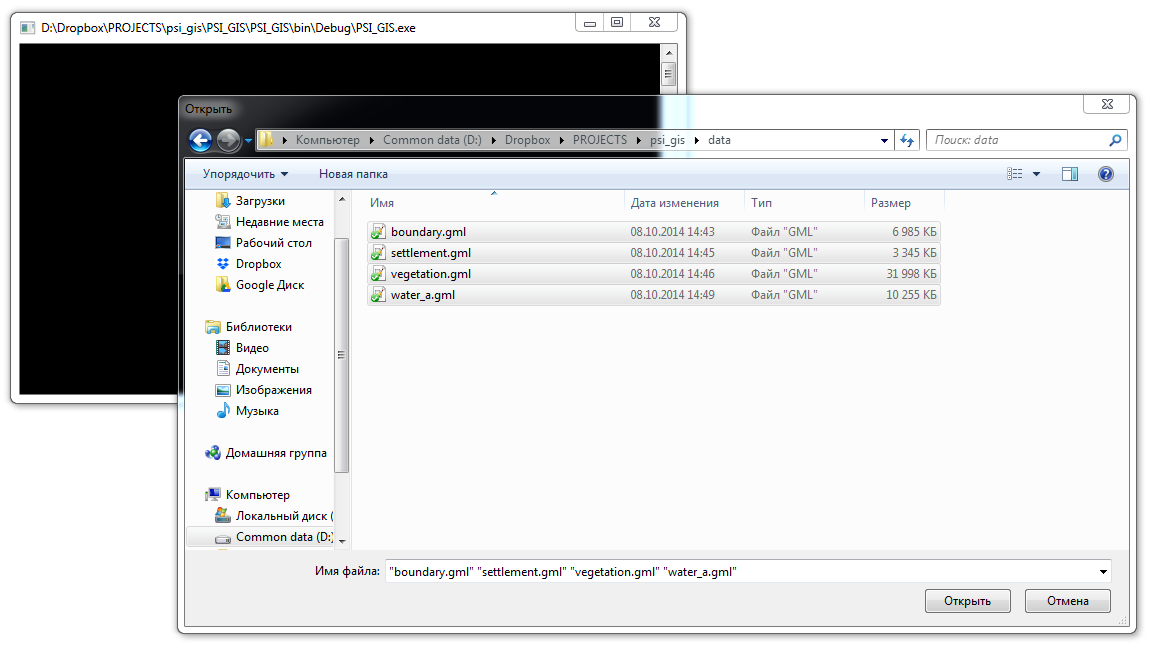
\includegraphics[width=1\textwidth]{dialog.png}
    \caption{Интерфейс ввода данных}
    \label{fig:dialog}
\end{figure}

\subsection{Объектная модель}
\label{}

\begin{center}
\begin{tikzpicture}
\umlclass[x=4,y=-13]{Vertex}{
  X, Y : double
}{
 distance(v : Vertex) : double
}
\umlclass[x=-5,y=-13]{Line}{
  a, b : Vertex
}{
 intersects(l : Line) : bool \\
 length() : double
}
\umlclass[x=-0.5,y=-7]{Poly}{
  vert : Vertex[]
}{
 Poly(XML : string) \\
 toXML() : XElement \\
 clearPath(v0, v1 : int) : bool \\
 reduce(poly : Poly) : Poly
}
\umlclass[x=4]{OuterPoly}{
  IP : Poly[] \\
  cutsGraph : int[,]
}{
 lineAllowed(line : Line) : bool \\
 shortestN2(p0, p1 : int) : int[2] \\
 buildPath(p0, p1 : int) : void \\
 Prim() : void \\
 unite() : void
}
\umlclass[x=-5]{FeatureMember}{
  pols : list<Poly> \\
  context : XElement \\
}{
 FeatureMember(node : XElement) \\
 toXML() : XElement
}
\umlunicompo[]{Line}{Vertex}
\umlunicompo[geometry=-|, anchor1=-20]{Poly}{Vertex}
\umlunicompo[geometry=|-, stereo=list]{FeatureMember}{Poly}
\umlunicompo[geometry=|-, stereo=array, anchor2=20]{OuterPoly}{Poly}
\end{tikzpicture}
\end{center}

\begin{itemize}
\item \textbf{Vertex}: базовый класс, представляет точку на плоскости.
\item \textbf{Line}: представляет отрезок. Состоит из двух объектов Vertex. Содержит методы для измерения длины и проверки пересечения с другим отрезком.
\item \textbf{Poly}: Общее представление многоугольника. Состоит из объектов Vertex. Реализует методы прямого и обратного преобразования в GML-элемент (Poly, toXML). Метод ClearPath проверяет, можно ли соединить две вершины многоугольника, не пересекая при этом его сторон. Метод reduce реализует алгоритм, описанный в \ref{task2}.
\item \textbf{OuterPoly}: Представляет многосвязную область. Состоит из внешней границы, представляемой объектом Poly, и массива многоугольников (IP), представляющих <<дыры>>. Метод lineAllowed проверяет, можно ли провести внутри области отрезок, не пересекающий сторон ни одного из составляющих ее многоугольников. Метод shortestN2 определяет кратчайший отрезок, соединяющий два многоугольника внутри области. Метод unite реализует алгоритм, описанный в \ref{task1} при помощи методов buildPath для построения полного графа соединений и Prim для алгоритма Прима.
\item \textbf{FeatureMember}: хранит метаданные областей, не имеющие отношения к их геометрии. Реализует ввод и вывод в GML.
\end{itemize}

\subsection{Пример работы}
\label{}

См. рис. \ref{fig:nocuts} и \ref{fig:result}.

\begin{figure}[!htb]
    \centering
    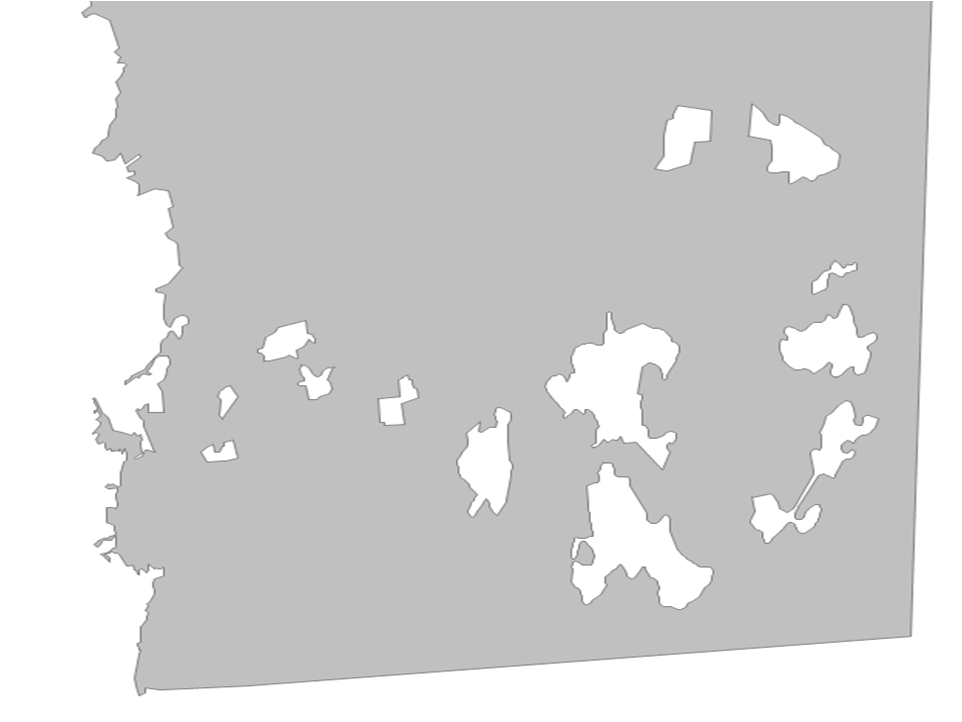
\includegraphics[width=1\textwidth]{nocuts.png}
    \caption{Визуализация фрагмента входного файла}
    \label{fig:nocuts}
\end{figure}

\begin{figure}[!htb]
    \centering
    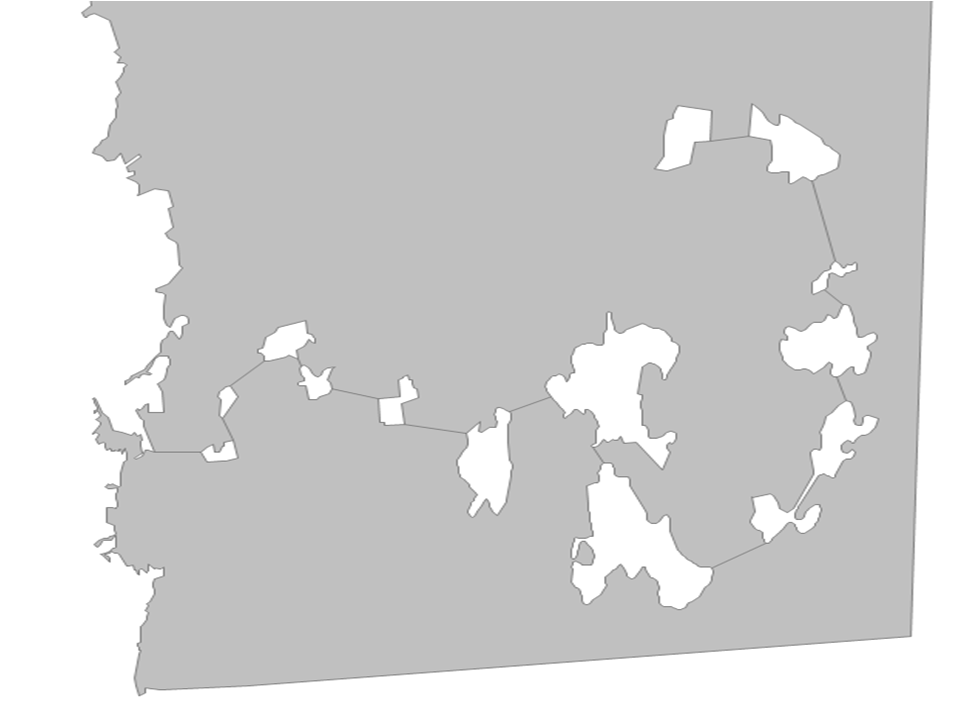
\includegraphics[width=1\textwidth]{result.png}
    \caption{Результат преобразования фрагмента файла}
    \label{fig:result}
\end{figure}